\chapter{Running the tool}
\label{chap:3}

In this chapter, few steps before running the tool are explained. Then, the process to run the tool is shortly shown and the expected output is described.

\section{Steps before running the tool}
First, to be able to run the tool properly, all the input files, as explained in Chapter \ref{chap:1}, have to be altered as needed by the user and imported in the same folder as the Python scrips. \\

Second, the input data table has to be made before running the tool. This is can be done by running the function in the script called Create\_Dummy\_Database.py with the input file (Login\_Data.txt). This will create a dummy database with 3 input rows. It is possible to run the code from the command line by calling the file name, or from Python by calling: \\ Create\_Dummy\_Database.Create\_dummy\_input\_Database('Login\_Data.txt')\\ after importing Create\_Dummy\_Database. \\

Third, it is recommended to make a new user for MySQL database instead of using the preprogrammed one. Creating a new user can be done trough the MySQL workbench or also the command prompt or MySQL shell, as explained in this article \cite{user}. The user should be granted all the privileges and should be created at the localhost. Then the new user name and password should be updated in the input file (Login\_Data.txt).\\

Fourth, at this point, the mode of the instrument is left blank in the input table. This is where the wavelength would be determined. This means that the wavelength (microns) needs to be specified, either as value or a list of values, to determine brightness at these values. This is done in the script called Run\_Script\_Tomake\_Database.py by giving values to a variable lambdaMu.



\section{How to run the tool}
When all the previous steps has been taken, the tool can be run. This can be done from the script called Run\_Script\_Tomake\_Database.py. As there are 4 functions, user can choose a one of them. This is done by uncommenting the desired line and updating the inputs for the function. This refers to the date, which determines which data needs to be rerun as outdated. The names of the input files or the lamdaMu input does not need to be changed unless the user renamed them. 

\section{Expected outputs}
After the tool was run, the output should be a multiple tables in the MySQL database called ISPY. Each of these tables gives the asteroids expected in the specified field of view at the specified moment. For each asteroid, some physical characteristics and calculated brightness are given as well as can be seen in Figure \ref{fig:2} and \ref{fig:3}. The table names are taken as the OBD\_id from the INPUT\_Table. \\

\begin{figure}[h]
    \centering
    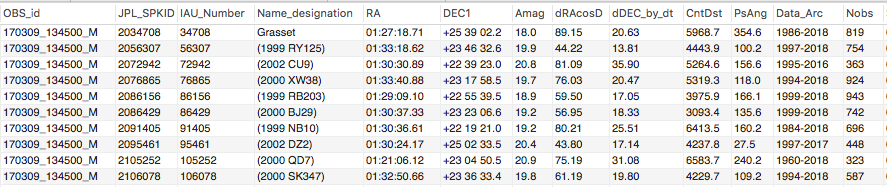
\includegraphics[width=1\textwidth]{Figures/Output1.png}
    \caption{The expected Output table, part 1}
    \label{fig:2}
\end{figure}

\begin{figure}[h]
    \centering
    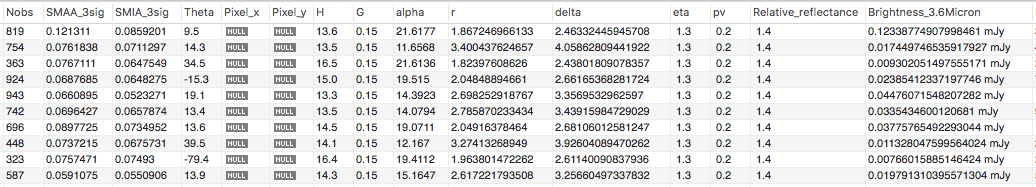
\includegraphics[width=1\textwidth]{Figures/Output2.png}
    \caption{The expected Output table, part 2}
    \label{fig:3}
\end{figure}

There are 26 columns, plus column or columns for brightness, this number depends on the number of values for wavelengths.
\begin{itemize}
    \item OBD\_id is a unique id made up of the field of view, date and instrument as specified in the input table as well. This is the foreign key for each table. Foreign keys help to cross-reference related data across tables.
    \item JPL\_SPKID is a unique numeric id within JPL's SPICE system for the object.
    \item IAU\_Number is the object's IAU number, if given.
    \item Name\_Designation is the object's IAU name (if assigned) or primary designation. 
    \item RA is the predicted astrometric right-ascension (light-time corrected) of the object in ICRF/J2000 cooordinates. Units: HH MM SS.ff (hours, minutes, and seconds of time)
    \item DEC1 is the predicted astrometric declination (light-time aberrated) of the object 
in ICRF/J2000 coordinates. Units: DG MN SC.ff (degrees, minutes, and seconds 
of arc)
    \item Amag is the apparent visual magnitude of the object.
    \item dRAcosD is the instantaneous rate of change of astrometric right-ascension at the
observation time. Units: ARCSECONDS PER HOUR
    \item dDEC\_by\_dt is the instantaneous rate of change of astrometric declination. 
Units: ARCSECONDS PER HOUR
    \item CntDst is the angular distance of the object from the centroid of the field of view.
Units: ARCSECONDS
    \item PsAng is the position angle of the object relative to the field centroid, measured
counter-clockwise (CCW) from Celestial North direction (e.g. line of constant 
right-ascension). Units: DEGREES
    \item Data\_Arc are the years spanned by the astrometry included in the object's orbit solution.
If less than one year, the number of days in the data arc is displayed.
    \item Nobs is the number of observations included in the object's orbit solution.
    \item SMAA\_3sig is the angular width of the 3-sigma error ellipse semi-major axis in plane-of-sky. Units: ARCSECONDS
    \item SMIA\_3sig is the angular width of the 3-sigma error ellipse semi-minor axis in plane-of-sky. Units: ARCSECONDS.\textbf{}
    \item Theta is the orientation angle of the error ellipse in plane-of-sky; the clockwise angle from the direction of increasing RA to the semi-major axis of the error ellipse, in the direction of increasing DEC.  Units: DEGREES.
    \item Pixel\_x are the pixels in x direction at which the asteroid should appear. 
    \item Pixel\_y are the pixels in y direction at which the asteroid should appear. 
    \item H is the absolute magnitude of the asteroid.
    \item G is the slope parameter.
    \item alpha is the Sun-Target-Observer angle; the interior vertex angle at
target center formed by a vector to the apparent center of the Sun at
reflection time on the target and the apparent vector to the observer at
print-time. Slightly different from true PHASE ANGLE (requestable separately)
at the few arcsecond level in that it includes stellar aberration on the
down-leg from target to observer.  Units: DEGREES
    \item r is Heliocentric range
of the target center at the instant light seen by the observer at print-time
would have left the target center (print-time minus down-leg light-time).
The Sun-to-target distance traveled by a ray of light emanating from the
center of the Sun that reaches the target center point at some instant and
is recordable by the observer one down-leg light-time later at print-time.
Units: AU 
    \item delta is range of target center with respect
to the observer at the instant light seen by the observer at print-time would
have left the target center (print-time minus down-leg light-time); the
distance traveled by a light ray emanating from the center of the target and
recorded by the observer at print-time. 
Units: AU 
    \item eta is the beaming parameter of the asteroid.
    \item pv is the albedo of the asteroid. 
    \item Relative\_reflectance is the relative reflectance of the asteroid.
    \item Brightness\_xMicron is the calculated brightness of the asteroid, both due to thermal emission and reflected brightness. 
    
\end{itemize}
At this time, there is no calculation for Pixel x and y included in the code.\\


Each table has a comment which gives user the information about input data for this table, observation date, instrument, mode and the field of view. This comment can be found when running a command in the command prompt or MySQL shell: \\
SELECT TABLE\_COMMENT FROM information\_schema.TABLES WHERE TABLE\_NAME = 'table name';\\
To see the table the following command can be used:\\
SELECT * from table name;\\
To examine the created tables in more ways, the user is recommend to read more about MySQL databases \cite{mysql}.

